\begin{figure}[!htbp]  % float page; will try to use its own page
  \centering
   %%%%%%%%%%%%%%%%%%%%%%%%%%%%%% 
    \begin{tcolorbox}[colback=white,colframe=black!30,boxrule=0.6pt,left=2mm,right=2mm,top=2mm,bottom=2mm,width=\linewidth]
    \footnotesize \textbf{Excerpt from \cite{abu2023rare}:}
    \begin{quote}\footnotesize
    A 57-year-old man recently diagnosed with lepromatous leprosy was confirmed with skin biopsy and had been on treatment (rifampicin/clofazimine/dapsone) for 2 months before admission; he was presented to the hospital with complaints of abdominal distension, constipation, vomiting, and a 10-kg weight loss. On examination, the patient was vitally stable. He had evidence of peripheral lymphadenopathy with a distended abdomen and a positive shifting dullness. A computed tomography scan of his abdomen showed mural thickening of the terminal ileum with significantly enlarged mesenteric lymph nodes, mesenteric fat stranding, and intra-abdominal free fluid, suggesting abdominal granulomatous infection or neoplastic process.
    \dots 
    
    The patient was planned for consolidation by autologous bone marrow transplant. Unfortunately, with the recurrent bacteremia and sepsis that accompanied the patient’s course due to his immunocompromised state, he was re-admitted to the medical ICU for severe sepsis and multiorgan failure and passed away around 6 months after his initial diagnosis with NHL, despite maintaining a remission status.
    \end{quote}
    \end{tcolorbox}
    %\vspace{2pt}
    %%%%%%%%%%%%%%%%%%%%%%%%%%%%%% 
  % Row 1
  \begin{subfigure}[!]{0.45\linewidth}\centering
    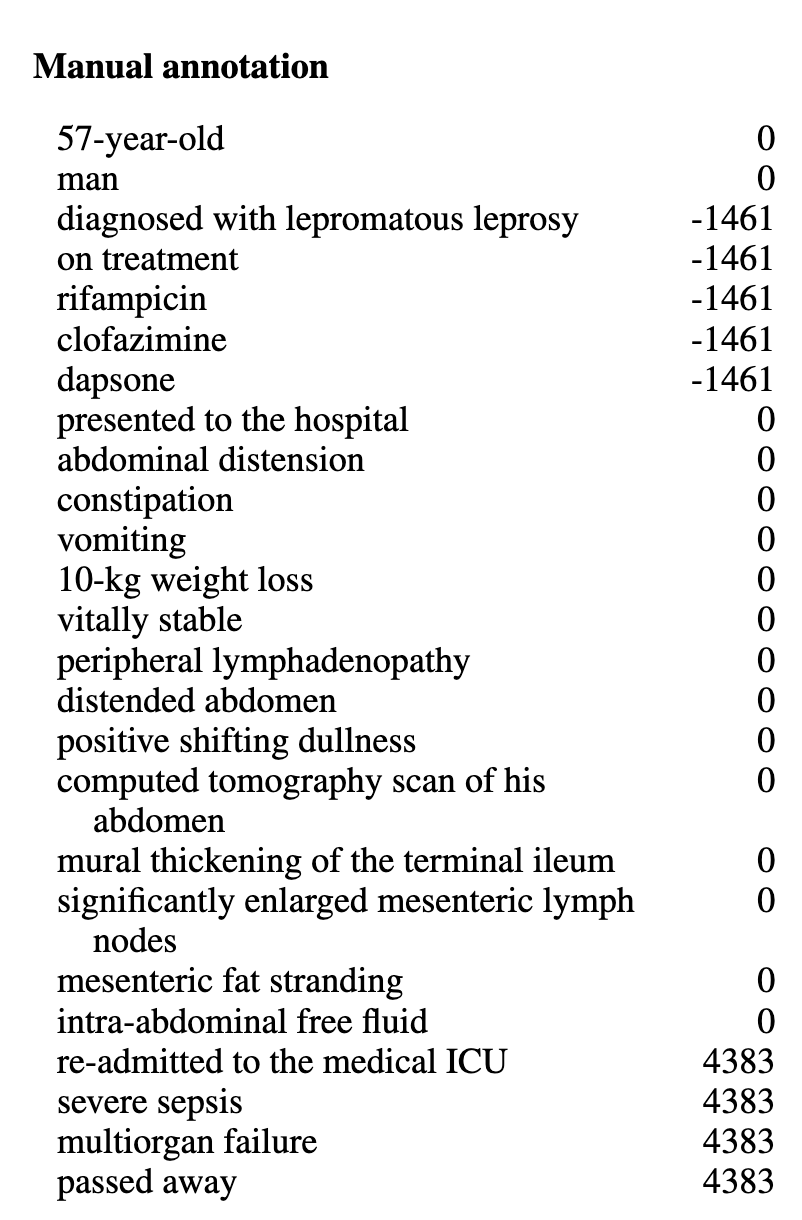
\includegraphics[width=0.9\linewidth]{Scientific_data/Supplementary/example_TTS_for_paper/manual.png}
    %\caption{...}\label{fig:a}
  \end{subfigure}\hfill
  \begin{subfigure}[!htbp]{0.45\linewidth}\centering
    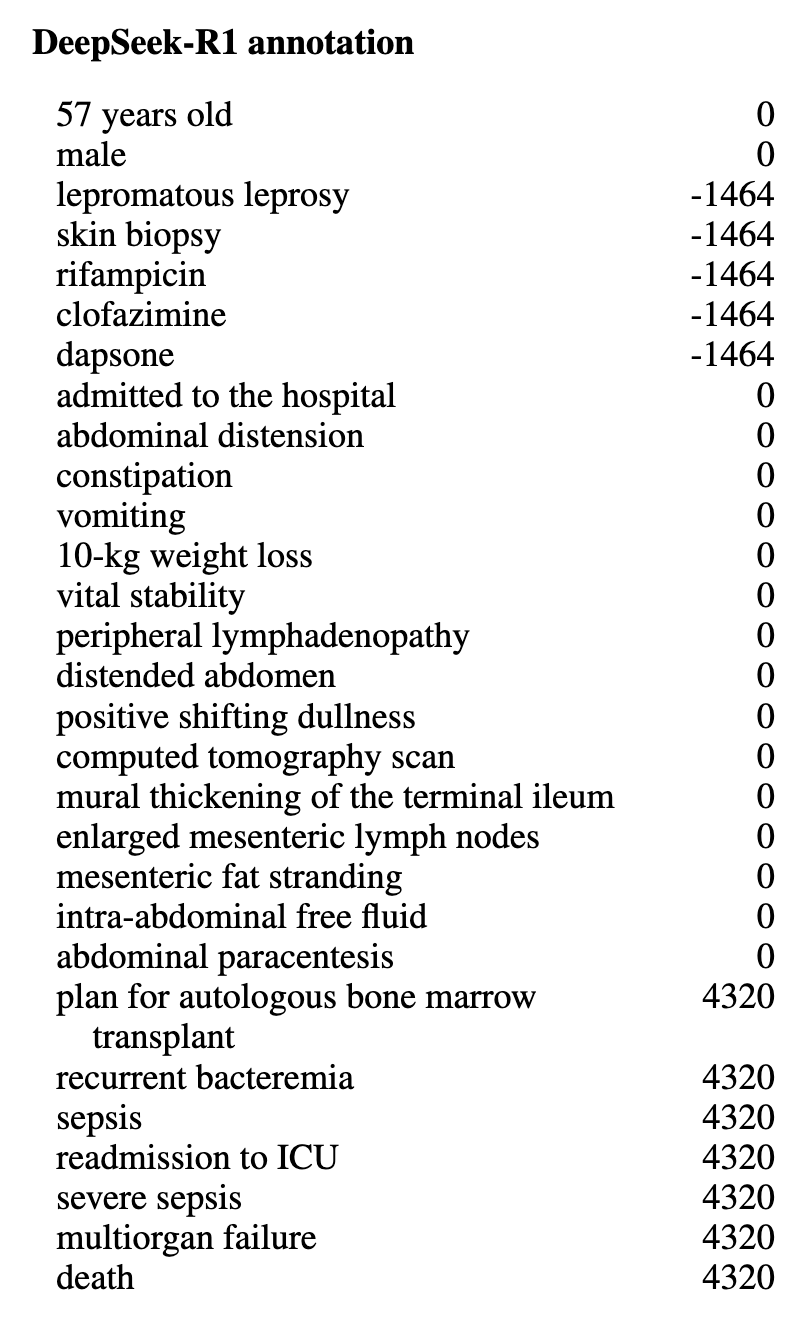
\includegraphics[width=0.9\linewidth]{Scientific_data/Supplementary/example_TTS_for_paper/DeepSeekR1.png}
    %\caption{...}\label{fig:b}
  \end{subfigure}

  %\vspace{6pt}

  % Row 2
  \begin{subfigure}[!htbp]{0.45\linewidth}\centering
    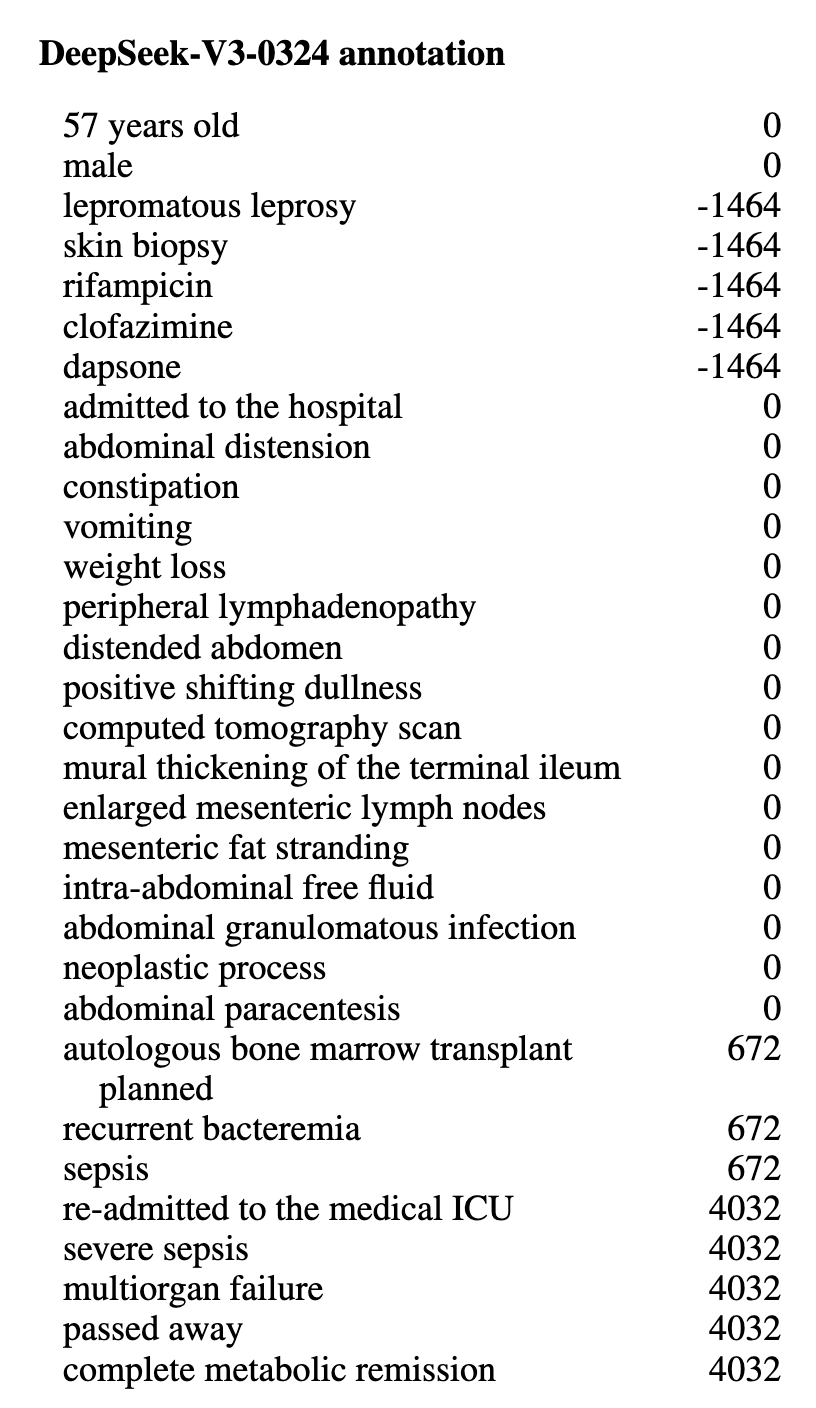
\includegraphics[width=0.9\linewidth]{Scientific_data/Supplementary/example_TTS_for_paper/DeepSeekV3.png}
    %\caption{...}\label{fig:c}
  \end{subfigure}\hfill
  \begin{subfigure}[!htbp]{0.45\linewidth}\centering
    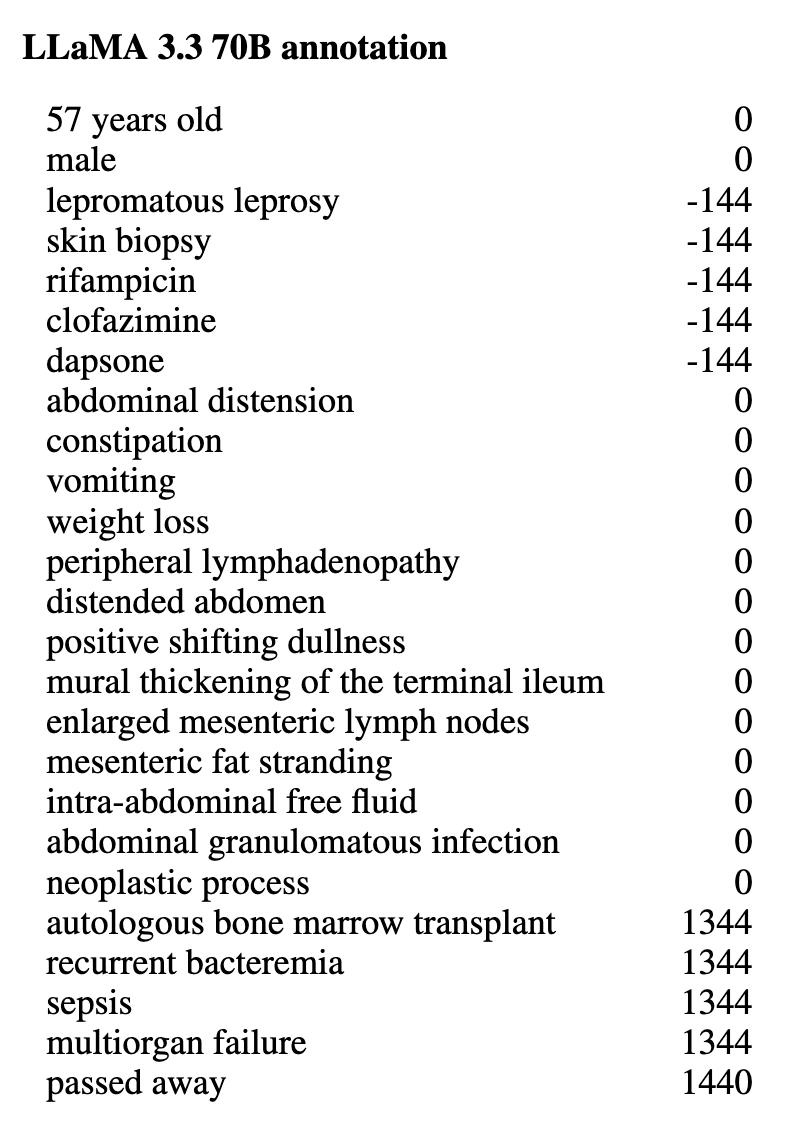
\includegraphics[width=0.9\linewidth]{Scientific_data/Supplementary/example_TTS_for_paper/L3370B.png}
    %\caption{...}\label{fig:d}
  \end{subfigure}
  %\caption{Overall caption for panels (a)–(d).}\label{fig:eight}
\end{figure}

%%%%%%%%%%%%%%%%%%%%%%%%%%%%%%%%%%%%%

\begin{figure}[!htbp]
  \centering
  % Row 1
  \begin{subfigure}[!htbp]{0.45\linewidth}\centering
    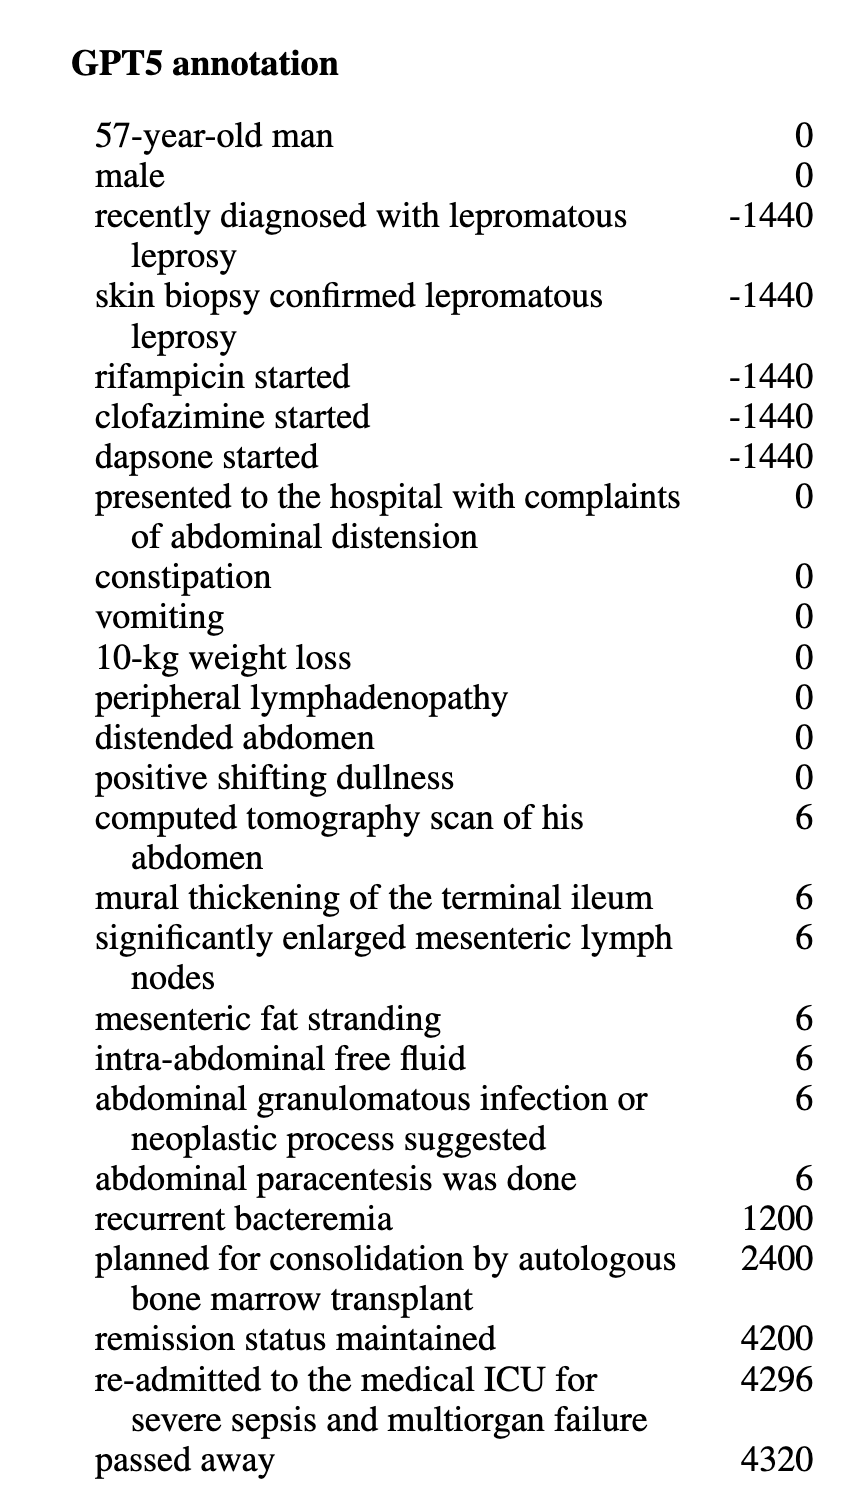
\includegraphics[width=0.9\linewidth]{Scientific_data/Supplementary/example_TTS_for_paper/GPT5.png}
    %\caption{...}\label{fig:e}
  \end{subfigure}\hfill
  \begin{subfigure}[!htbp]{0.45\linewidth}\centering
    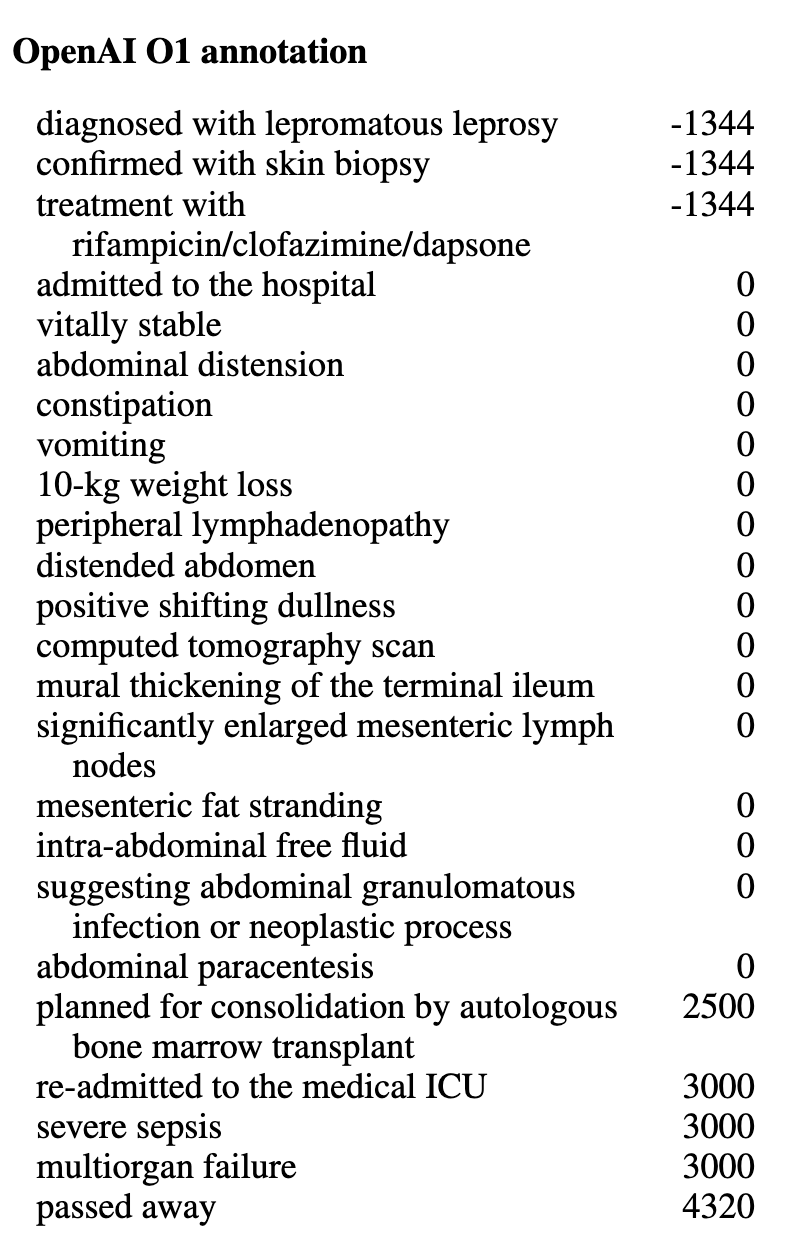
\includegraphics[width=0.9\linewidth]{Scientific_data/Supplementary/example_TTS_for_paper/O1.png}
    %\caption{...}\label{fig:f}
  \end{subfigure}

  \vspace{2pt}

  % Row 2
  \begin{subfigure}[!htbp]{0.45\linewidth}\centering
    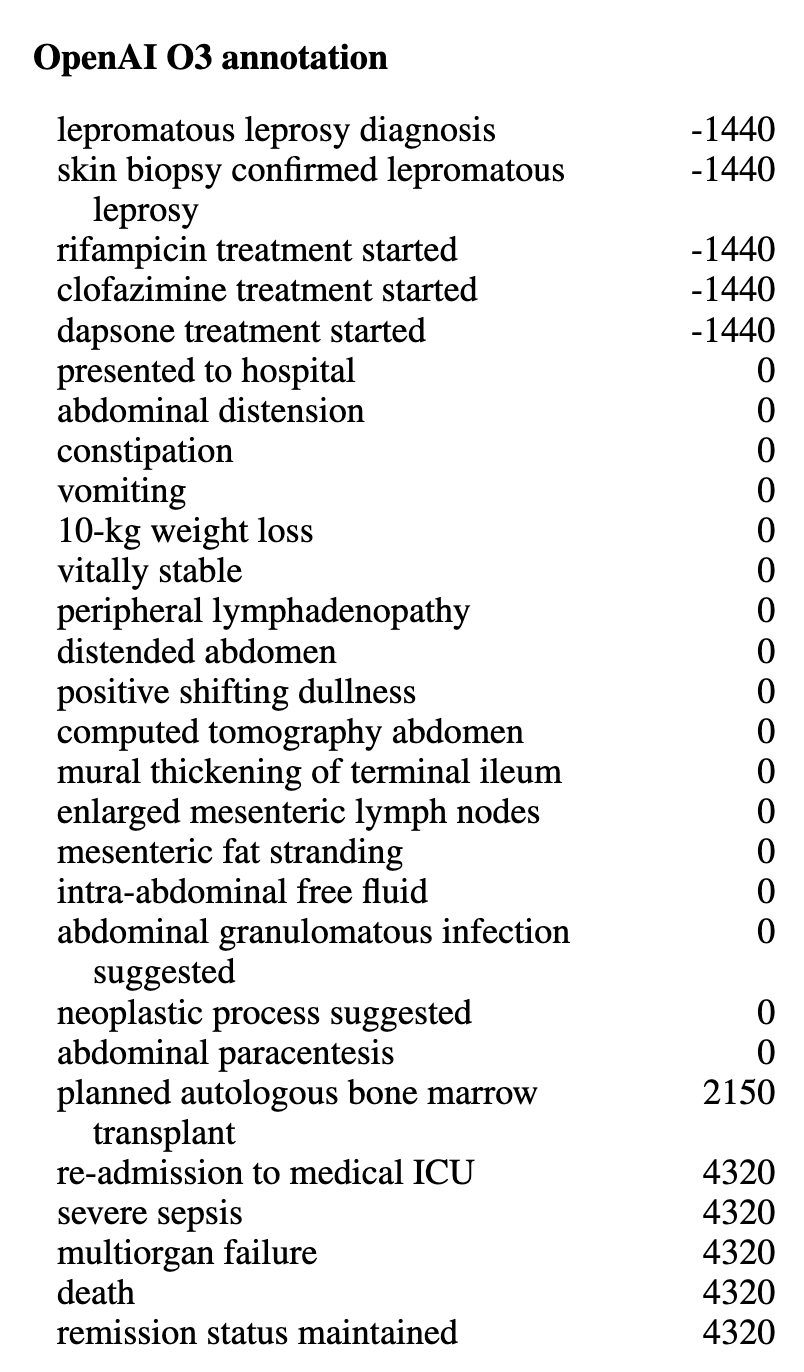
\includegraphics[width=0.9\linewidth]{Scientific_data/Supplementary/example_TTS_for_paper/O3.png}
    %\caption{...}\label{fig:g}
  \end{subfigure}\hfill
  \begin{subfigure}[!htbp]{0.45\linewidth}\centering
    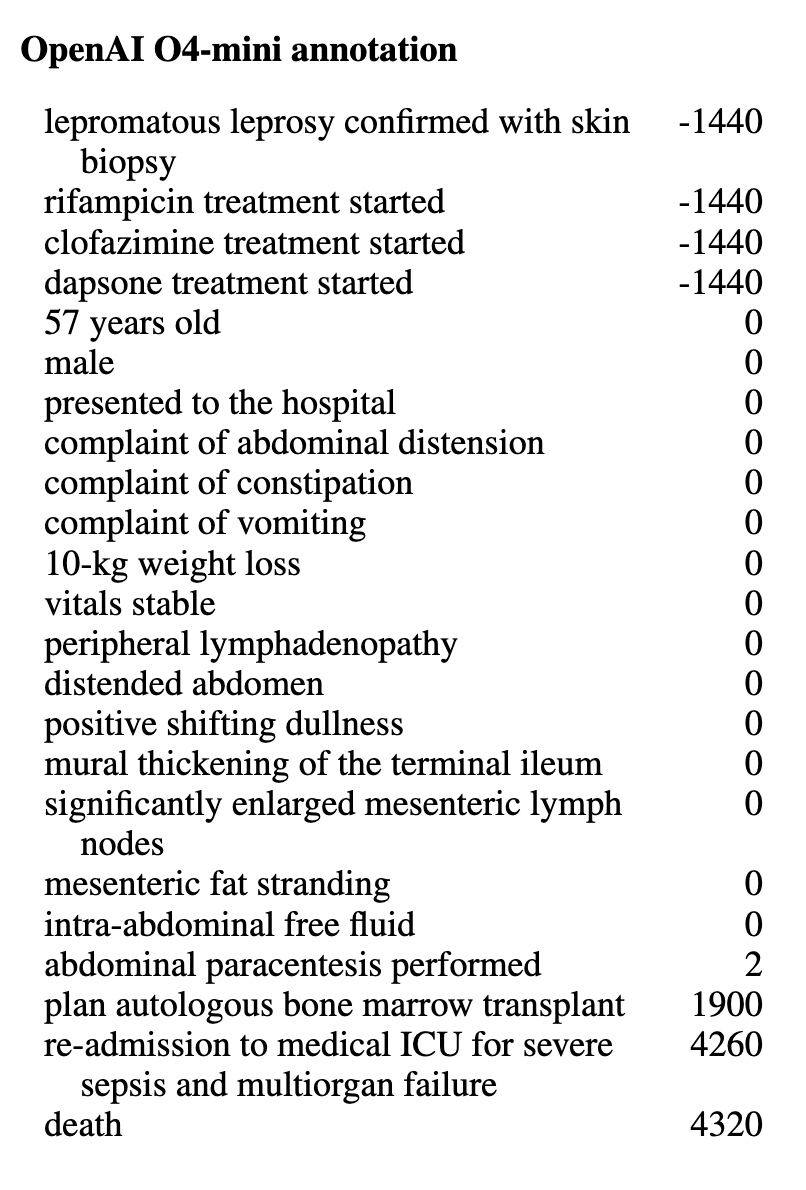
\includegraphics[width=0.9\linewidth]{Scientific_data/Supplementary/example_TTS_for_paper/O4mini.png}
    %\caption{...}\label{fig:h}
  \end{subfigure}

\caption{Comparison of temporal annotations generated by several LLMs for a representative case report (PMC10629858). The figure contrasts manual annotations with model-generated event–time
sequences, highlighting differences in event granularity, phrasing, duplicate event generation, and temporal normalization (e.g., variation in converting narrative expressions such as ``two
months before admission’’ into hour offsets). Long-range timestamp assignments (e.g., for transplant planning, ICU readmission, and death) show the greatest variability across models, whereas the overall ordering of major clinical events is largely preserved. This example illustrates characteristic
differences in how LLMs interpret, segment, and temporally anchor clinical narratives.}
  \label{fig:compare_llm_annotations}
  \vspace{-3mm}
\end{figure}


%%%%%%%%%%%%%%%%%%%%%%%%%%%%%%%%%%%%%%%%%
%%%%%%%%%%%%%%%%%%%%%%%%%%%%%%%%%%%%%%%%%

% \begin{figure*}[t]
% \centering

% % ---------------------------------------------------
% % Top: Excerpt box
% % ---------------------------------------------------
% \begin{tcolorbox}[
%   colback=white,
%   colframe=black!30,
%   boxrule=0.6pt,
%   left=2mm,right=2mm,top=2mm,bottom=2mm,
%   width=\linewidth
% ]
% \footnotesize \textbf{Excerpt from \cite{abu2023rare}:}
% \begin{quote}\footnotesize
% A 57-year-old man recently diagnosed with lepromatous leprosy was confirmed with skin biopsy 
% and had been on treatment (rifampicin/clofazimine/dapsone) for 2 months before admission; he 
% presented to the hospital with complaints of abdominal distension, constipation, vomiting, and 
% a 10-kg weight loss. On examination, the patient was vitally stable. He had evidence of peripheral 
% lymphadenopathy with a distended abdomen and a positive shifting dullness. A computed tomography 
% scan of his abdomen showed mural thickening of the terminal ileum with significantly enlarged 
% mesenteric lymph nodes, mesenteric fat stranding, and intra-abdominal free fluid, suggesting 
% abdominal granulomatous infection or neoplastic process. \dots

% The patient was planned for consolidation by autologous bone marrow transplant. Unfortunately, 
% with recurrent bacteremia and sepsis due to his immunocompromised state, he was re-admitted 
% to the medical ICU for severe sepsis and multiorgan failure and passed away around 6 months 
% after his initial diagnosis with NHL.
% \end{quote}
% \end{tcolorbox}

% \vspace{6pt}

% % ---------------------------------------------------
% % Grid of 8 subfigures (4 rows × 2 columns)
% % ---------------------------------------------------

% % Row 1
% \begin{subfigure}[t]{0.45\textwidth}
% \centering
% 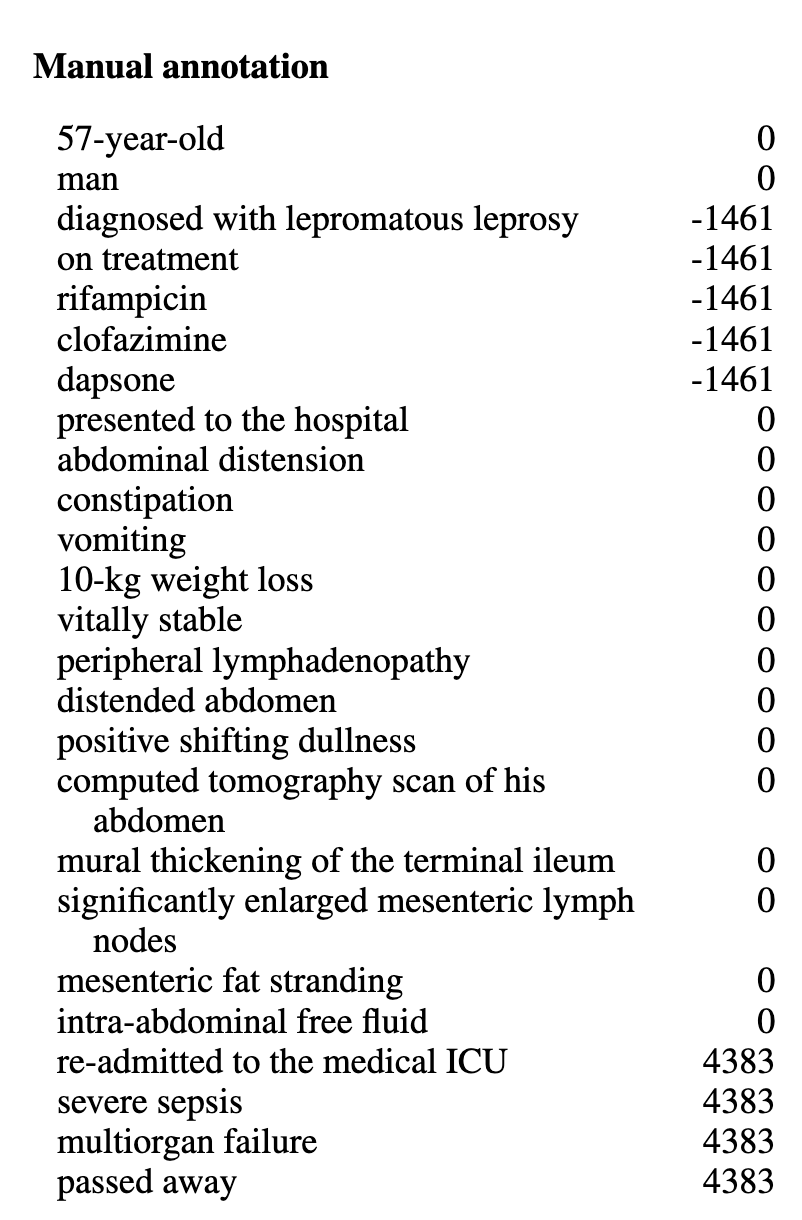
\includegraphics[width=0.95\linewidth]{Scientific_data/Supplementary/example_TTS_for_paper/manual.png}
% \caption*{Manual annotation}
% \end{subfigure}
% \hfill
% \begin{subfigure}[t]{0.45\textwidth}
% \centering
% 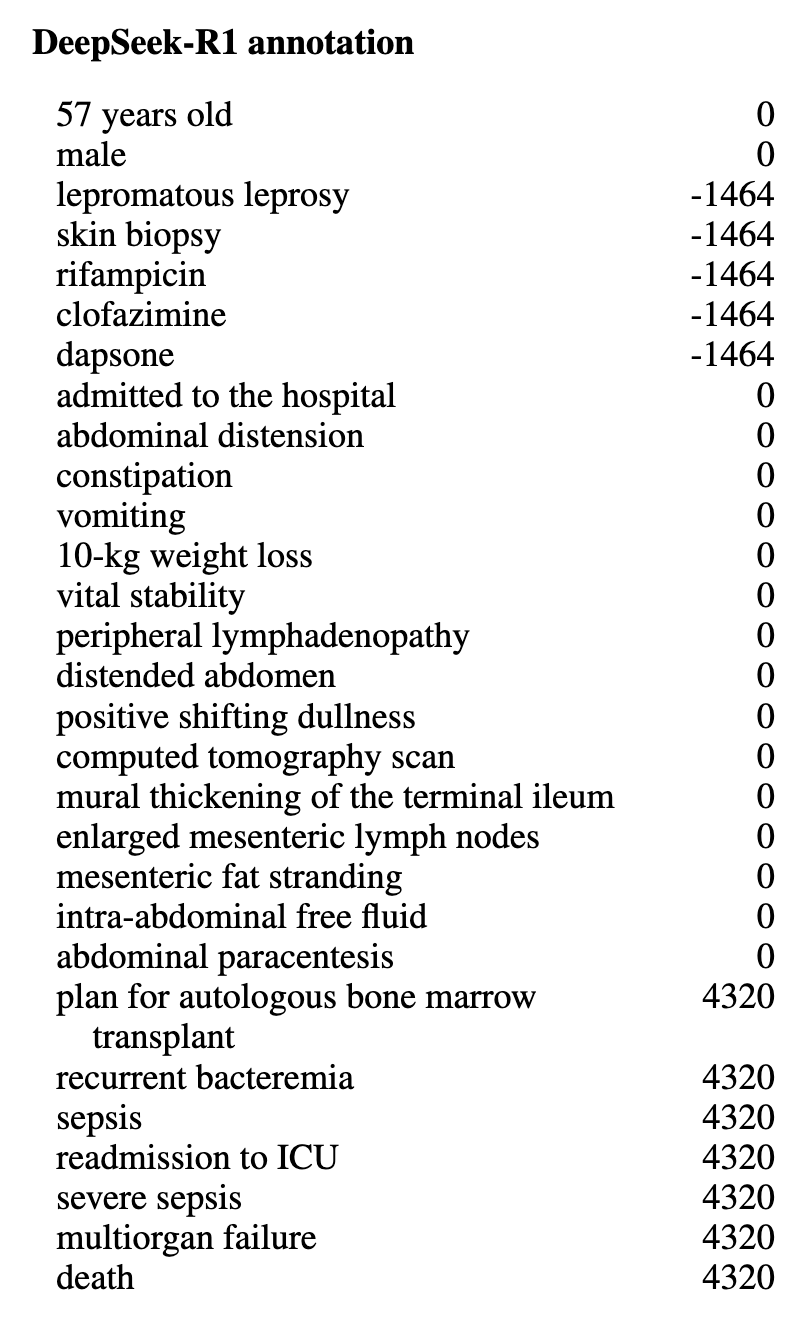
\includegraphics[width=0.95\linewidth]{Scientific_data/Supplementary/example_TTS_for_paper/DeepSeekR1.png}
% \caption*{\texttt{DeepSeek-R1}}
% \end{subfigure}

% \vspace{4pt}

% % Row 2
% \begin{subfigure}[t]{0.45\textwidth}
% \centering
% 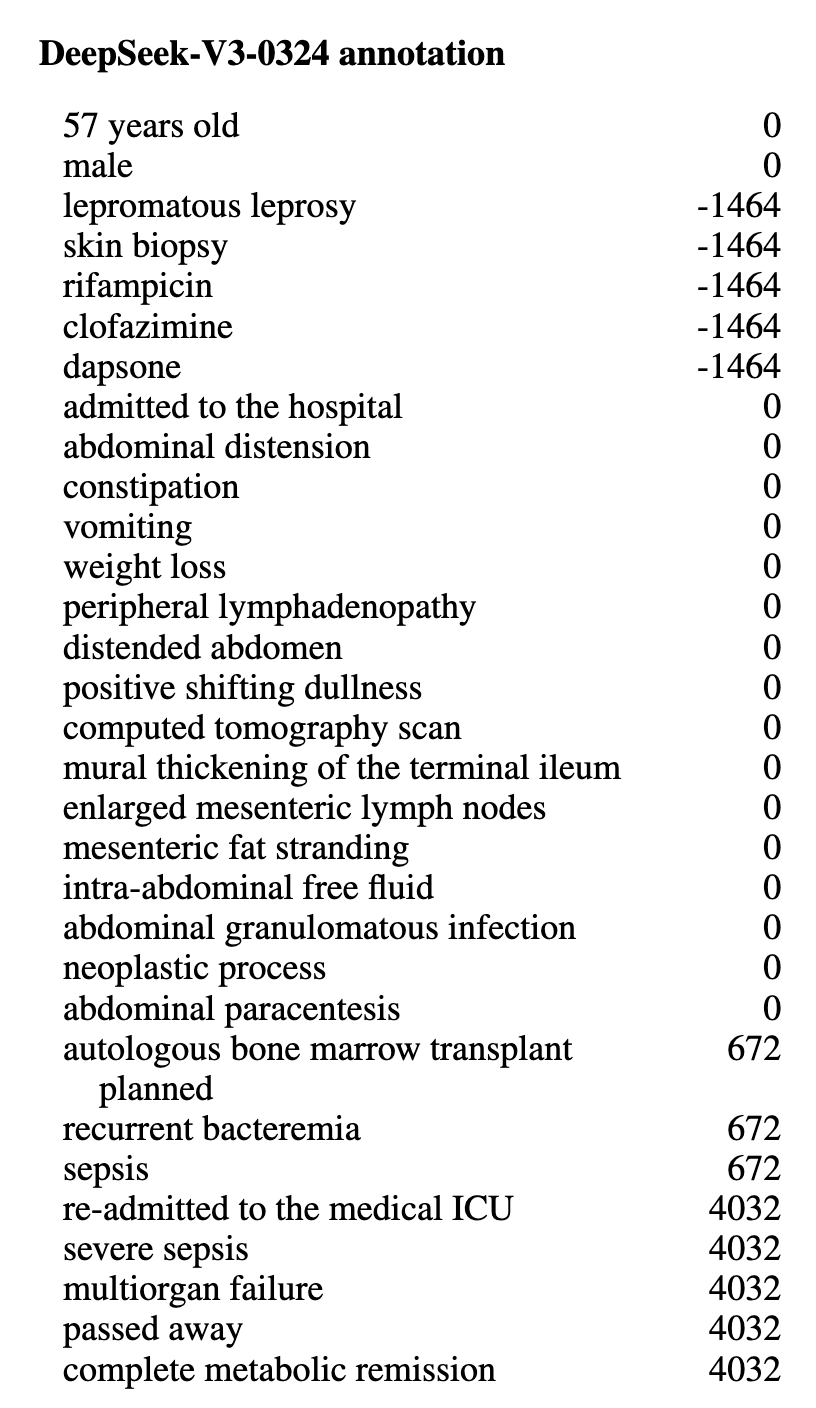
\includegraphics[width=0.95\linewidth]{Scientific_data/Supplementary/example_TTS_for_paper/DeepSeekV3.png}
% \caption*{\texttt{DeepSeek-V3-0324}}
% \end{subfigure}
% \hfill
% \begin{subfigure}[t]{0.45\textwidth}
% \centering
% 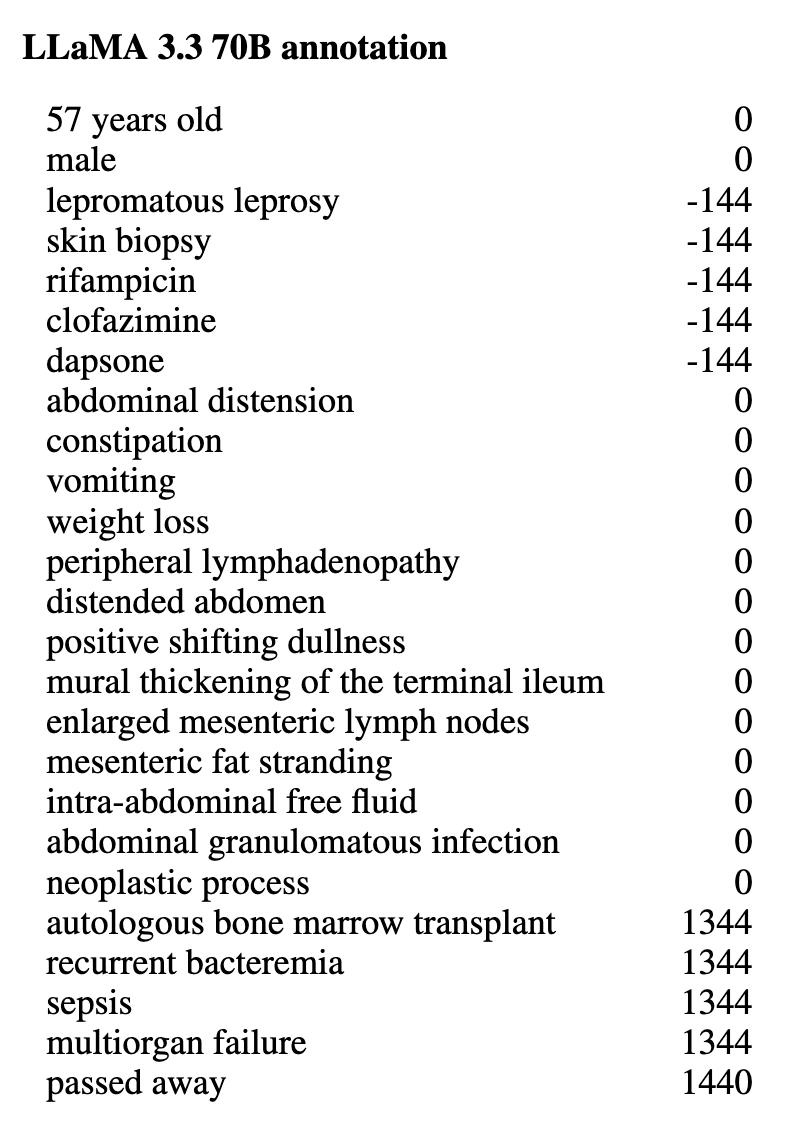
\includegraphics[width=0.95\linewidth]{Scientific_data/Supplementary/example_TTS_for_paper/L3370B.png}
% \caption*{\texttt{LLaMA~3.3~70B}}
% \end{subfigure}

% \vspace{4pt}

% % Row 3
% \begin{subfigure}[t]{0.45\textwidth}
% \centering
% 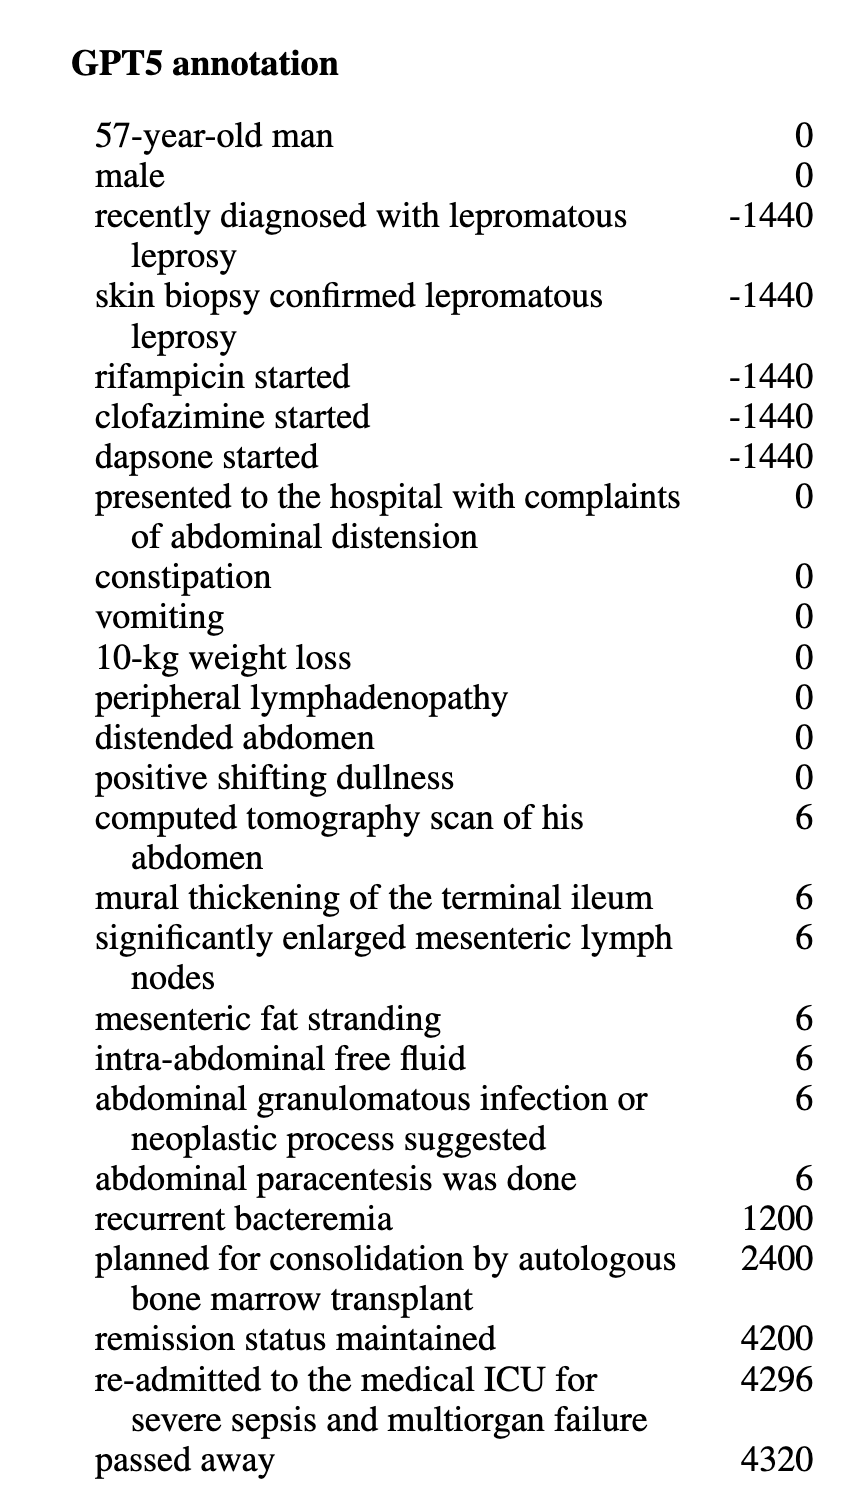
\includegraphics[width=0.95\linewidth]{Scientific_data/Supplementary/example_TTS_for_paper/GPT5.png}
% \caption*{\texttt{GPT5}}
% \end{subfigure}
% \hfill
% \begin{subfigure}[t]{0.45\textwidth}
% \centering
% 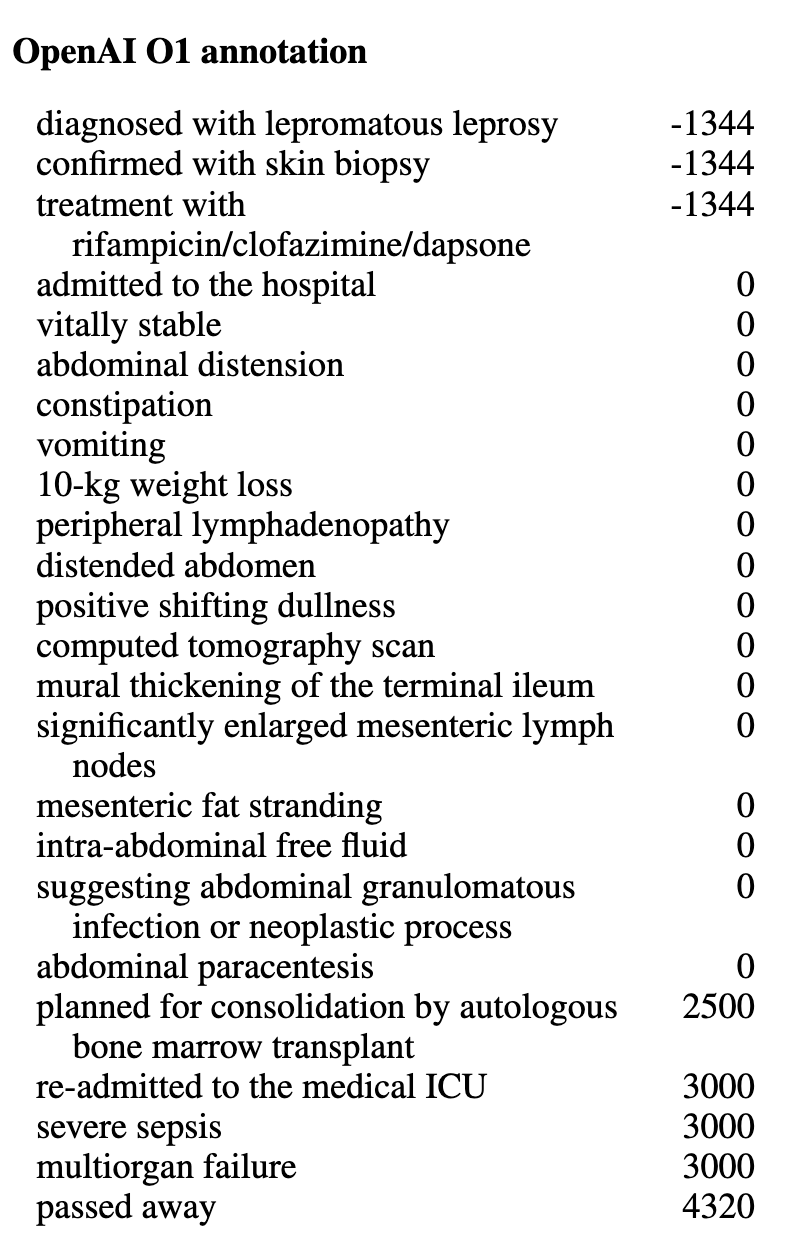
\includegraphics[width=0.95\linewidth]{Scientific_data/Supplementary/example_TTS_for_paper/O1.png}
% \caption*{\texttt{O1}}
% \end{subfigure}

% \vspace{4pt}

% % Row 4
% \begin{subfigure}[t]{0.45\textwidth}
% \centering
% 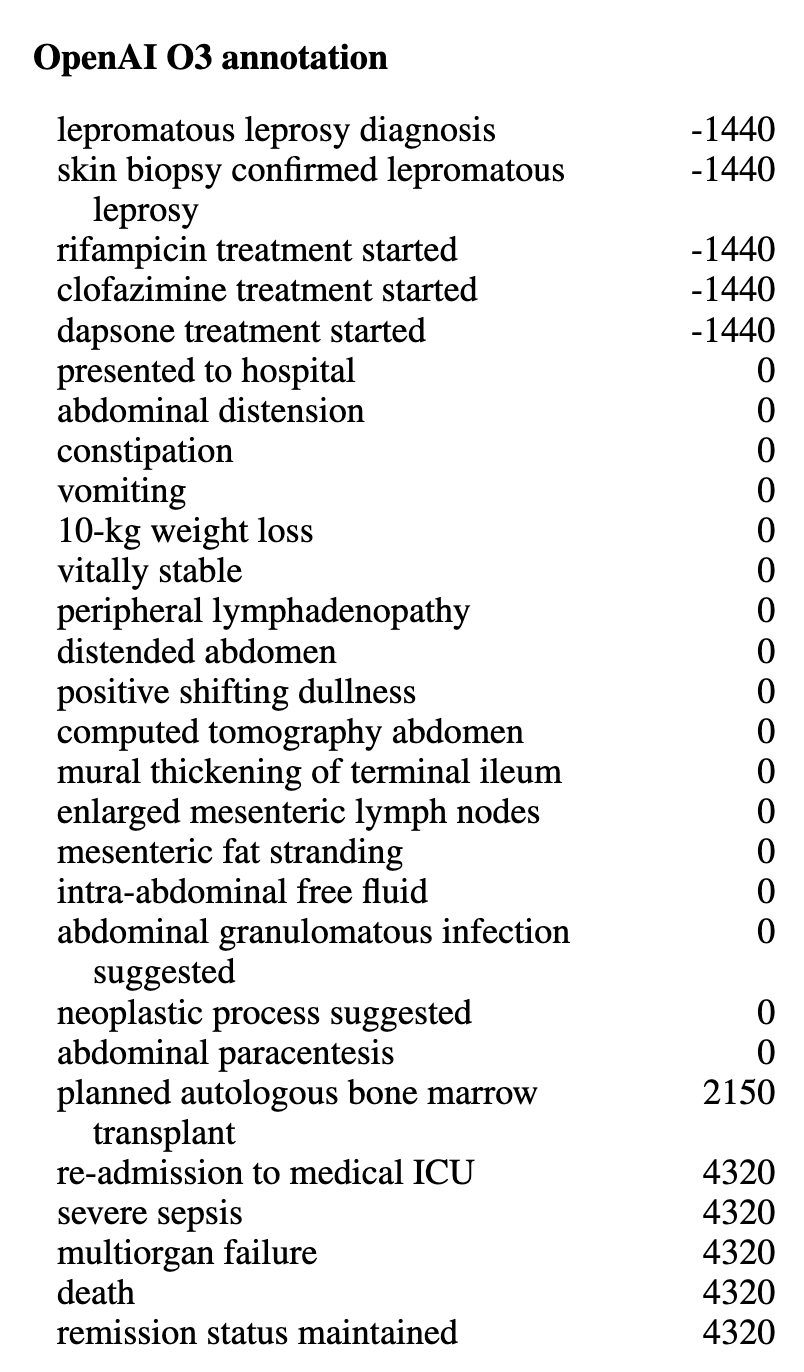
\includegraphics[width=0.95\linewidth]{Scientific_data/Supplementary/example_TTS_for_paper/O3.png}
% \caption*{\texttt{O3}}
% \end{subfigure}
% \hfill
% \begin{subfigure}[t]{0.45\textwidth}
% \centering
% 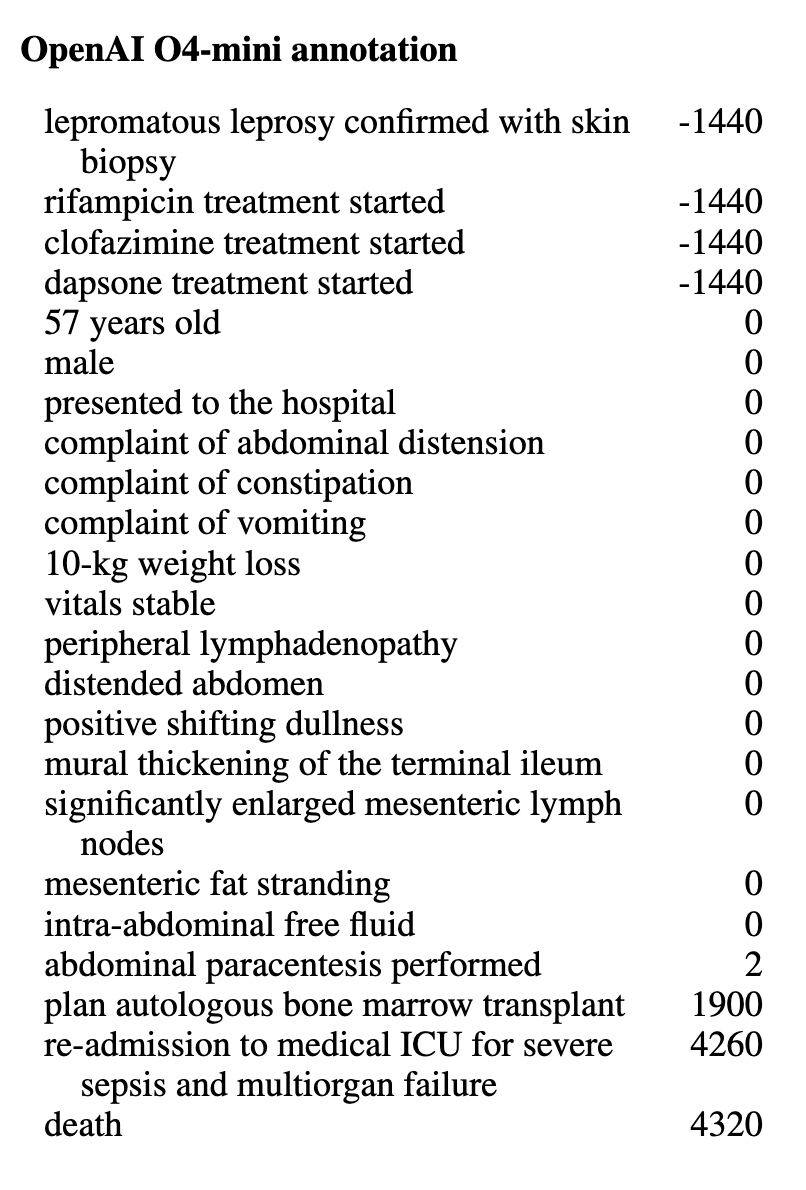
\includegraphics[width=0.95\linewidth]{Scientific_data/Supplementary/example_TTS_for_paper/O4mini.png}
% \caption*{\texttt{O4-mini}}
% \end{subfigure}

% % ---------------------------------------------------
% % Caption + Label
% % ---------------------------------------------------
% \caption{
% Comparison of temporal annotations generated by several LLMs for a representative case report  (PMC10629858). The figure contrasts manual annotations with model-generated event--time sequences, highlighting differences in event granularity, phrasing, duplicate event generation, and  temporal normalization (e.g., variation in converting narrative expressions such as  ``two months before admission'' into hour offsets). Long-range timestamp assignments  (e.g., for transplant planning, ICU readmission, and death) exhibit the greatest variability across models, whereas the overall ordering of major clinical events is largely preserved. 
% This example illustrates characteristic differences in how LLMs interpret, segment, and temporally anchor clinical narratives.
% }
% \label{fig:compare_llm_annotations}

% \vspace{-2mm}
% \end{figure*}
